\documentclass[11pt,a4paper]{article}

\usepackage[a4paper,margin=25mm]{geometry}
\usepackage[T1]{fontenc}
\usepackage[utf8]{inputenc}
\usepackage{lmodern}
\usepackage{microtype}
\usepackage{parskip}
\usepackage{xcolor}
\usepackage{graphicx}
\usepackage{float}
\usepackage{tikz}
\usetikzlibrary{arrows.meta,positioning}
\usepackage{booktabs}
\usepackage{tabularx}
\usepackage{enumitem}
\usepackage{hyperref}
\usepackage{listings}

\definecolor{ink}{HTML}{1F2937}
\definecolor{blue}{HTML}{1D4ED8}
\definecolor{muted}{HTML}{4B5563}
\definecolor{codebg}{HTML}{F8FAFC}

\hypersetup{
  colorlinks=true,
  linkcolor=blue,
  urlcolor=blue,
  pdftitle={Search Engine Optimization Project Proposal},
  pdfauthor={Python Learning Hub Team}
}
\urlstyle{same}
\graphicspath{{figures/}}
\setlist{leftmargin=*,itemsep=3pt,topsep=4pt}
\setlength{\emergencystretch}{3em}
\lstset{
  basicstyle=\ttfamily\small,
  backgroundcolor=\color{codebg},
  frame=single,
  breaklines=true,
  showstringspaces=false,
  columns=fullflexible
}

\title{Search Engine Optimization\\[0.35em]\large Project Proposal}
\author{SEO Python Hub Team}
\date{13 September 2026}

\begin{document}

% --------------------------------------------------
% PHYSICAL PAGE 1: CENTERED COVER PAGE
% --------------------------------------------------
\begin{titlepage}
  \thispagestyle{empty}
  \centering
  \vspace*{\fill}

  {\LARGE\bfseries SEO Python Hub \par}
  \vspace{0.35em}
  {\Large Project Proposal\par}

  \vspace{1.5cm}

  {\large\bfseries Search Engine Optimization \par}

  \vspace{1cm}

  {\itshape A structured proposal for a discoverable Python learning platform\par}

  \vspace{1cm}


  \vspace*{\fill}
\end{titlepage}

% --------------------------------------------------
% PHYSICAL PAGE 2: TABLE OF CONTENTS
% --------------------------------------------------
\pagenumbering{gobble}
\begingroup
  \small
  \setlength{\parskip}{0pt}
  \tableofcontents
\endgroup
\clearpage

% --------------------------------------------------
% PHYSICAL PAGE 3: MAIN CONTENT, NUMBERED 1
% --------------------------------------------------
\pagenumbering{arabic}
\setcounter{page}{1}

\section{Introduction}

\textbf{SEO Python Hub: A Search-Engine-Optimized Python Learning Platform} is a
structured learning and community website designed to make high-quality Python
education easy to discover through search engines. The platform combines
server-rendered public content with a richer authenticated application for
learning progress and community participation.

The project name is intentionally related to search engine optimization: public
topics, tutorials, guides, categories, and roadmap pages will be designed as
useful, indexable resources rather than as content that is available only after a
client-side application loads.

\section{Problem Statement}

Python learning resources are distributed across many websites and often provide
an incomplete path from beginner concepts to practical projects. Learners may
find isolated tutorials, but they can struggle to judge quality, follow a logical
sequence, save useful material, and continue learning after returning to the site.

The platform also has a technical discovery problem. If educational content is
hidden behind a client-side application, search engines and first-time visitors
may not receive useful content immediately. A solution is therefore needed that
offers crawlable public pages, clear information architecture, fast navigation,
and richer tools for signed-in users without creating two separate backends or
duplicating business rules.

\section{Objectives}

The project will pursue the following objectives:

\begin{enumerate}
  \item provide a beginner-to-advanced Python learning roadmap;
  \item publish clear topics, tutorials, guides, examples, categories, and tags;
  \item make public educational content searchable, shareable, and indexable;
  \item support registration, authentication, progress tracking, and bookmarks;
  \item provide public discussions with authenticated participation;
  \item expose a documented, versioned API for interactive application features;
  \item implement semantic HTML, clean URLs, metadata, canonical links, a sitemap,
        and crawler rules;
  \item provide a responsive and accessible user interface;
  \item evaluate the system through functional, SEO, performance, usability, and
        content-quality testing; and
  \item keep the application maintainable through shared services, repositories,
        schemas, and a staged implementation plan.
\end{enumerate}

\section{Stakeholders (Users) and GUI Users}

\subsection{Stakeholders}

\begin{tabularx}{\linewidth}{@{}p{.23\linewidth}X@{}}
\toprule
\textbf{Stakeholder} & \textbf{Needs and responsibilities}\\
\midrule
Visitor & Discover, browse, search, and read public Python learning content without
an account.\\
Learner & Register, continue along the roadmap, record progress, save bookmarks,
and participate in discussions.\\
Content administrator & Create and update topics, tutorials, guides, categories,
tags, publication state, and SEO metadata.\\
Moderator & Review discussions, manage reports, and protect the quality and safety
of community content.\\
Search engine & Receive accessible, server-rendered pages with stable URLs,
metadata, internal links, sitemap information, and accurate structured data.\\
Development and operations team & Maintain the shared backend, database, deployment
workflow, monitoring, testing, and security controls.\\
\bottomrule
\end{tabularx}

\subsection{GUI users}

The graphical user interface will support two groups of human users:

\begin{itemize}
  \item \textbf{Public GUI users:} visitors and learners who use the home page,
        search, roadmap, topic pages, tutorials, guides, and discussions.
  \item \textbf{Authenticated GUI users:} learners and administrators who use the
        dashboard, profile, progress, bookmarks, richer discussions, and protected
        administrative workflows.
\end{itemize}

The public GUI must remain useful with JavaScript disabled. HTMX may enhance small
interactions, but it must not be the only way to read or navigate the core content.

\section{System Panel}

\subsection{Two-experience model}

The system is one product with two deliberate presentation layers:

\begin{itemize}
  \item \textbf{Public website:} Jinja2 renders crawlable HTML for the home page,
        roadmap, categories, tags, tutorials, guides, topics, discussions, and
        search results. HTMX can add small progressive interactions.
  \item \textbf{Application panel:} Flutter Web provides authenticated dashboards,
        progress views, bookmarks, statistics, notifications, and richer workflows
        below the \texttt{/app/} path.
\end{itemize}

FastAPI remains the single HTTP boundary. Both presentation layers call shared
application services and repositories, and neither frontend accesses PostgreSQL
directly.

\clearpage
\subsection{Logical architecture}

\begin{figure}[htbp]
  \centering
  \resizebox{0.97\linewidth}{!}{%
  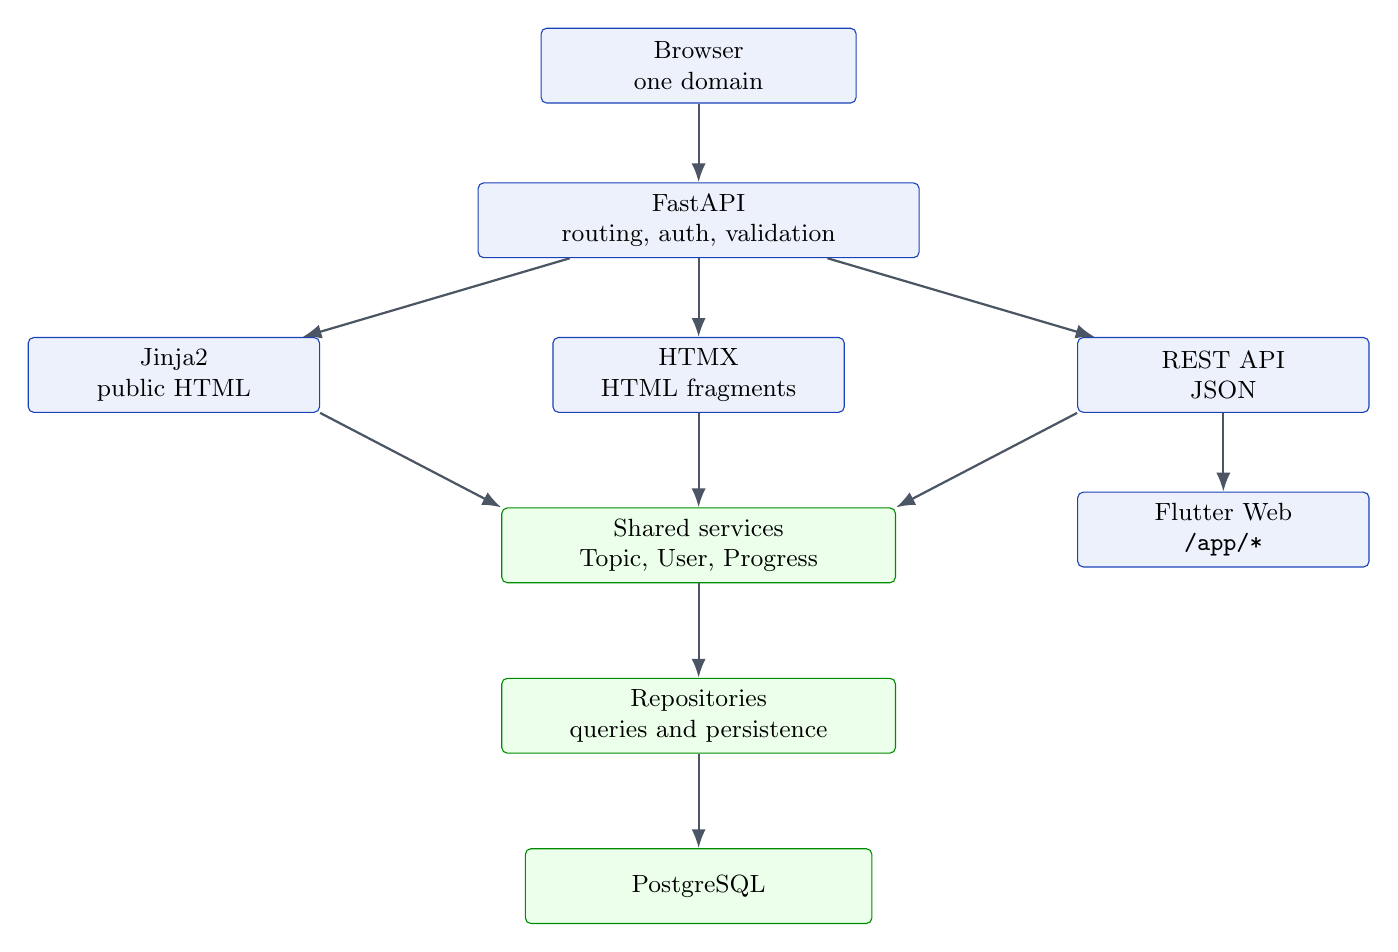
\begin{tikzpicture}[
    node distance=1.15cm and 1.55cm,
    logicalbox/.style={
      draw=blue!85!black,
      fill=blue!8,
      rounded corners=2pt,
      minimum height=0.95cm,
      minimum width=3.7cm,
      align=center,
      font=\small
    },
    servicebox/.style={
      draw=green!55!black,
      fill=green!8,
      rounded corners=2pt,
      minimum height=0.95cm,
      minimum width=5.0cm,
      align=center,
      font=\small
    },
    arrow/.style={-{Latex[length=2.4mm]}, thick, draw=muted}
  ]
    \node[logicalbox, minimum width=4.0cm] (browser) {Browser\\one domain};
    \node[logicalbox, minimum width=5.6cm, below=1.0cm of browser]
      (fastapi) {FastAPI\\routing, auth, validation};

    \node[logicalbox, below left=1.0cm and 2.0cm of fastapi]
      (jinja) {Jinja2\\public HTML};
    \node[logicalbox, below=1.0cm of fastapi]
      (htmx) {HTMX\\HTML fragments};
    \node[logicalbox, below right=1.0cm and 2.0cm of fastapi]
      (rest) {REST API\\JSON};
    \node[logicalbox, below=1.0cm of rest]
      (flutter) {Flutter Web\\\texttt{/app/*}};

    \node[servicebox, below=1.2cm of htmx]
      (services) {Shared services\\Topic, User, Progress};
    \node[servicebox, below=1.2cm of services]
      (repositories) {Repositories\\queries and persistence};
    \node[servicebox, minimum width=4.4cm, below=1.2cm of repositories]
      (postgres) {PostgreSQL};

    \draw[arrow] (browser) -- (fastapi);
    \draw[arrow] (fastapi) -- (jinja);
    \draw[arrow] (fastapi) -- (htmx);
    \draw[arrow] (fastapi) -- (rest);
    \draw[arrow] (jinja.south east) -- (services.north west);
    \draw[arrow] (htmx) -- (services);
    \draw[arrow] (rest.south west) -- (services.north east);
    \draw[arrow] (rest) -- (flutter);
    \draw[arrow] (services) -- (repositories);
    \draw[arrow] (repositories) -- (postgres);
  \end{tikzpicture}%
  }
  \caption{Logical architecture: one FastAPI boundary connects public HTML, HTMX,
  the REST API, Flutter Web, shared services, repositories, and PostgreSQL.}
  \label{fig:logical-architecture}
\end{figure}

\subsection{URL ownership}

The URL prefixes form an explicit routing contract:

\begin{tabularx}{\linewidth}{@{}p{.29\linewidth}p{.22\linewidth}X@{}}
\toprule
\textbf{Prefix or example} & \textbf{Owner} & \textbf{Purpose}\\
\midrule
\texttt{/}, \texttt{/roadmap} & Jinja2 & Public landing and roadmap pages.\\
\texttt{/topics/\{slug\}} & Jinja2 & Crawlable topic and tutorial content.\\
\texttt{/categories/\{slug\}} & Jinja2 & Category landing pages.\\
\texttt{/discussions/\{id\}} & Jinja2 & Public discussion pages.\\
\texttt{/search} & Jinja2 & Search form and server-rendered results.\\
\texttt{/web-components/...} & HTMX/Jinja2 & Small HTML fragments returned to public pages.\\
\texttt{/app/...} & Flutter Web & Authenticated client-side application routes.\\
\texttt{/api/v1/...} & FastAPI & JSON data and mutation contract.\\
\texttt{/ws/...} & FastAPI & Optional real-time features introduced later.\\
\bottomrule
\end{tabularx}

\subsection{Core request flow}

For a public topic such as \texttt{/topics/python-functions}, FastAPI dispatches to
the public router, the router calls \texttt{TopicService}, and the service reads
through \texttt{TopicRepository}. Jinja2 then receives the result and returns
complete HTML. A Flutter request such as \texttt{GET /api/v1/progress} follows the
same service and repository path, but FastAPI serializes the result as JSON.

The Flutter fallback is scoped below \texttt{/app}. It serves real generated assets
and returns the Flutter entry document for client-side routes such as
\texttt{/app/dashboard}; it must never catch public pages, API routes, HTMX
endpoints, or missing assets outside that prefix.

\subsection{Production deployment}

The current deployment model builds Flutter Web with \texttt{/app/} as its base
path, copies the generated artifact into \texttt{backend/app/flutter/web}, and
serves it from the same FastAPI deployment. The production topology is shown in
Figure~\ref{fig:production-topology}.

\subsubsection{Deployment workflow}

The release path from source control to the running application is summarized in
Figure~\ref{fig:deployment-workflow}.

\begin{figure}[H]
  \centering
  \resizebox{0.99\linewidth}{!}{%
  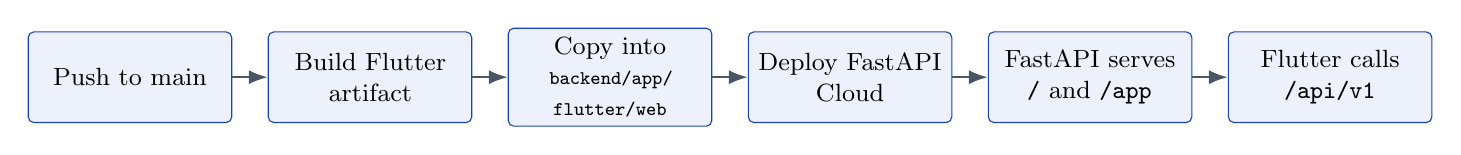
\begin{tikzpicture}[
    workflowbox/.style={
      draw=blue!85!black,
      fill=blue!8,
      rounded corners=2pt,
      minimum width=2.55cm,
      minimum height=1.15cm,
      text width=2.35cm,
      align=center,
      font=\small
    },
    arrow/.style={-{Latex[length=2.4mm]}, thick, draw=muted}
  ]
    \node[workflowbox] (push) {Push to main};
    \node[workflowbox, right=0.45cm of push]
      (build) {Build Flutter\\artifact};
    \node[workflowbox, right=0.45cm of build]
      (copy) {Copy into\\\texttt{\scriptsize backend/app/}\\\texttt{\scriptsize flutter/web}};
    \node[workflowbox, right=0.45cm of copy]
      (deploy) {Deploy FastAPI\\Cloud};
    \node[workflowbox, right=0.45cm of deploy]
      (serve) {FastAPI serves\\\texttt{/} and \texttt{/app}};
    \node[workflowbox, right=0.45cm of serve]
      (api) {Flutter calls\\\texttt{/api/v1}};

    \draw[arrow] (push) -- (build);
    \draw[arrow] (build) -- (copy);
    \draw[arrow] (copy) -- (deploy);
    \draw[arrow] (deploy) -- (serve);
    \draw[arrow] (serve) -- (api);
  \end{tikzpicture}%
  }
  \caption{Deployment workflow from the main branch to the FastAPI and Flutter Web
  runtime.}
  \label{fig:deployment-workflow}
\end{figure}

\section{Main Features}

The initial system will provide the following features:

\begin{enumerate}
  \item \textbf{Public learning library:} approximately 15--25 Python topics and
        5--10 tutorials or guides, with categories, tags, slugs, breadcrumbs,
        examples, and related-content navigation.
  \item \textbf{Roadmap and discovery:} a structured learning path, topic search,
        category pages, guide listings, useful no-result pages, and stable links.
  \item \textbf{Accounts and learner actions:} registration, secure login, progress
        tracking, bookmarks, activity history, and profile settings.
  \item \textbf{Discussions:} public questions and replies with authenticated
        participation, reporting, moderation state, and role-based controls.
  \item \textbf{Authenticated dashboard:} a Flutter Web interface for continuing
        learning, progress summaries, bookmarks, statistics, and richer workflows.
  \item \textbf{Administration:} content management, SEO metadata management,
        user management, reports, moderation, and basic statistics.
  \item \textbf{System quality:} semantic HTML, responsive layouts, accessible
        markup, useful 404 pages, health checks, automated tests, and documented
        deployment.
\end{enumerate}

\section{Technology Stack (Programming Language)}

\begin{tabularx}{\linewidth}{@{}p{.24\linewidth}p{.25\linewidth}X@{}}
\toprule
\textbf{Area} & \textbf{Technology} & \textbf{Purpose}\\
\midrule
Programming language & Python & Backend services, route handlers, tests, and deployment scripts.\\
Backend & FastAPI and Uvicorn & Routing, dependency injection, validation, authentication,
JSON endpoints, and API documentation.\\
Public interface & Jinja2 and HTMX & Fast server-rendered HTML and small progressive interactions.\\
Application GUI & Flutter Web and Dart & Rich authenticated navigation, dashboards, charts, and stateful workflows.\\
Database & PostgreSQL with asynchronous \texttt{asyncpg} queries & Durable storage for users, content, progress, bookmarks, and discussions.\\
Persistence boundary & Repositories and shared services & Keeps SQL and business rules out of route handlers and widgets.\\
Migrations & Alembic & Repeatable, reviewable database changes.\\
Caching and real time & Redis and WebSockets (later phases) & Selected read-heavy operations, notifications, chat, and scale features after validation.\\
Deployment & FastAPI Cloud & One production origin for public pages, API, and Flutter Web.\\
\bottomrule
\end{tabularx}

The Flutter source remains in \texttt{frontend/}; only its generated Web artifact is
copied to \texttt{backend/app/flutter/web}. The backend keeps database queries in
repositories, business rules in services, and API contracts in request and response
schemas.

\subsection{Implementation workflow}

The planned workflow is:

\begin{lstlisting}
python scripts/build_flutter.py
cd backend
uv run pytest
uv run fastapi deploy .
\end{lstlisting}

The build helper installs dependencies, builds with \texttt{--base-href /app/},
injects the compile-time \texttt{API\_BASE\_URL}, validates the generated output,
and copies it into the backend package. The same Git commit should release the
backend and the Flutter artifact.

\section{GUI Design}

The GUI will use a simple, content-first layout so that search visitors can reach
useful material quickly and authenticated users can move naturally into the richer
application panel.

\begin{tabularx}{\linewidth}{@{}p{.25\linewidth}X@{}}
\toprule
\textbf{Screen or component} & \textbf{Design proposal}\\
\midrule
Header & Project identity, roadmap link, topic categories, search field, and account actions.\\
Home page & Short value proposition, featured topics, learning roadmap entry point,
popular guides, and a clear call to continue learning.\\
Topic page & Breadcrumbs, title and summary, difficulty, structured content, examples,
progress/bookmark actions, related topics, and discussion entry point.\\
Roadmap & Ordered learning path with prerequisites, completion state, filters, and
links to public topic pages.\\
Learner dashboard & Progress summary, continue-learning card, bookmarks, activity
history, statistics, and notifications.\\
Administrator panel & Protected content, SEO metadata, user, report, moderation, and
basic analytics views.\\
Accessibility & Keyboard navigation, visible focus states, labelled controls, readable
contrast, semantic headings, responsive layouts, and useful error/empty states.\\
\bottomrule
\end{tabularx}

The public pages will be implemented with semantic server-rendered HTML. Flutter
will be used when client-side state, charts, filters, or multi-step interaction
provides clear value. This keeps the interface efficient without forcing every
feature into a single-page application.

\section{SEO Strategy}

SEO is a core product requirement rather than a final polishing step. The system
will apply the following strategy.

\subsection{On-page and technical SEO}

Every indexable page should provide:

\begin{itemize}
  \item a unique, descriptive title and meta description;
  \item one clear H1 and a logical heading hierarchy;
  \item a stable, readable, canonical URL;
  \item server-rendered content in the initial response;
  \item meaningful internal links between related topics;
  \item breadcrumbs where they clarify the content hierarchy;
  \item accurate structured data only when it describes the page; and
  \item a sitemap and \texttt{robots.txt} policy that reflect publication state.
\end{itemize}

\subsection{Content and information architecture}

Content will be organized around search intent and learning progression. Topic
pages will link to prerequisites, examples, tutorials, guides, categories, and
related topics. Titles, summaries, headings, slugs, and metadata will be reviewed
for clarity rather than generated as meaningless keyword lists. Public discussion
pages and useful search results will be available at ordinary URLs when they add
value to a visitor.

\subsection{Performance, accessibility, and measurement}

Fast server-rendered responses, optimized static assets, responsive layouts,
accessible markup, and useful error pages will support both users and crawlers.
The project will use functional tests, Lighthouse SEO and accessibility checks
targeting at least 90/100, a target performance score of at least 85/100,
content review, and usability testing with approximately 5--10 users. Search
rankings cannot be guaranteed; the measurable goal is to build technically sound,
useful pages that deserve to be found.

\subsection{Public route set}

The first public route set will include:

\begin{lstlisting}
GET /                 Home page
GET /roadmap          Learning roadmap
GET /topics/{slug}    Topic page
GET /tutorials        Tutorial listing
GET /guides           Guide listing
GET /search           Search page
GET /discussions      Public discussions
GET /sitemap.xml      Published-page sitemap
GET /robots.txt       Crawler rules
\end{lstlisting}

The guiding rule is simple: if a page is valuable to someone who has not signed
in, it should be a real Jinja2 URL. Flutter may link to it, but search engines
should not need to boot Flutter to read it.

\section{Limitations}

The first release is deliberately limited. It will not attempt to provide every
learning or community feature at once.

\begin{itemize}
  \item Initial content coverage is limited to approximately 15--25 topics and
        5--10 tutorials or guides.
  \item Quizzes, advanced analytics, extensive moderation dashboards, background
        jobs, Redis caching, WebSockets, chat, and expanded library coverage are
        not prerequisites for the first release.
  \item Payments, video hosting, live classes, native mobile applications, AI
        tutoring, online code execution, and guaranteed search rankings are outside
        the initial scope.
  \item Search visibility depends on content quality, competition, crawlability,
        site performance, authority, and ongoing maintenance; implementation alone
        cannot guarantee a ranking.
  \item Administrative and moderation processes will remain lightweight until the
        project has enough content and users to justify more complex tooling.
\end{itemize}

\section{Future Enhancements}

After the public learning workflow is stable, the project can be extended with:

\begin{enumerate}
  \item quizzes, exercises, certificates, and more detailed learning analytics;
  \item Redis caching, background jobs, search indexing, and performance scaling;
  \item WebSockets, notifications, chat, and richer community workflows;
  \item expanded administration, moderation dashboards, audit events, and reports;
  \item additional Python libraries, frameworks, projects, and structured learning
        tracks;
  \item native mobile applications using the same versioned API;
  \item carefully scoped AI-assisted explanations or recommendations; and
  \item secure online code execution after isolation, resource limits, and abuse
        controls have been designed and tested.
\end{enumerate}

The implementation roadmap should remain staged: public learning site first,
accounts and lightweight learner actions second, Flutter workflows third, and
discussions, administration, real-time features, and scale capabilities only when
the earlier foundations are validated.

\section{Conclusion}

SEO Python Hub will combine discoverable educational content with a richer
authenticated learning experience. FastAPI will provide one reliable application
boundary; Jinja2 and HTMX will preserve useful, search-friendly public pages; and
Flutter Web will support interactive workflows without creating a second
production backend. Shared services and repositories will keep both interfaces
consistent, while the staged roadmap keeps the initial release achievable.

The central design principle is: \textbf{one domain, one FastAPI backend, two
deliberate presentation layers, shared services, and an SEO-first public content
strategy}.

\end{document}
